\chapter{项目展示}

    \section{用户界面}
    制作了提供暗色系和暖色系两种主题。下图是用户使用时的界面:

    TODO(我截不了弦振动的图)
    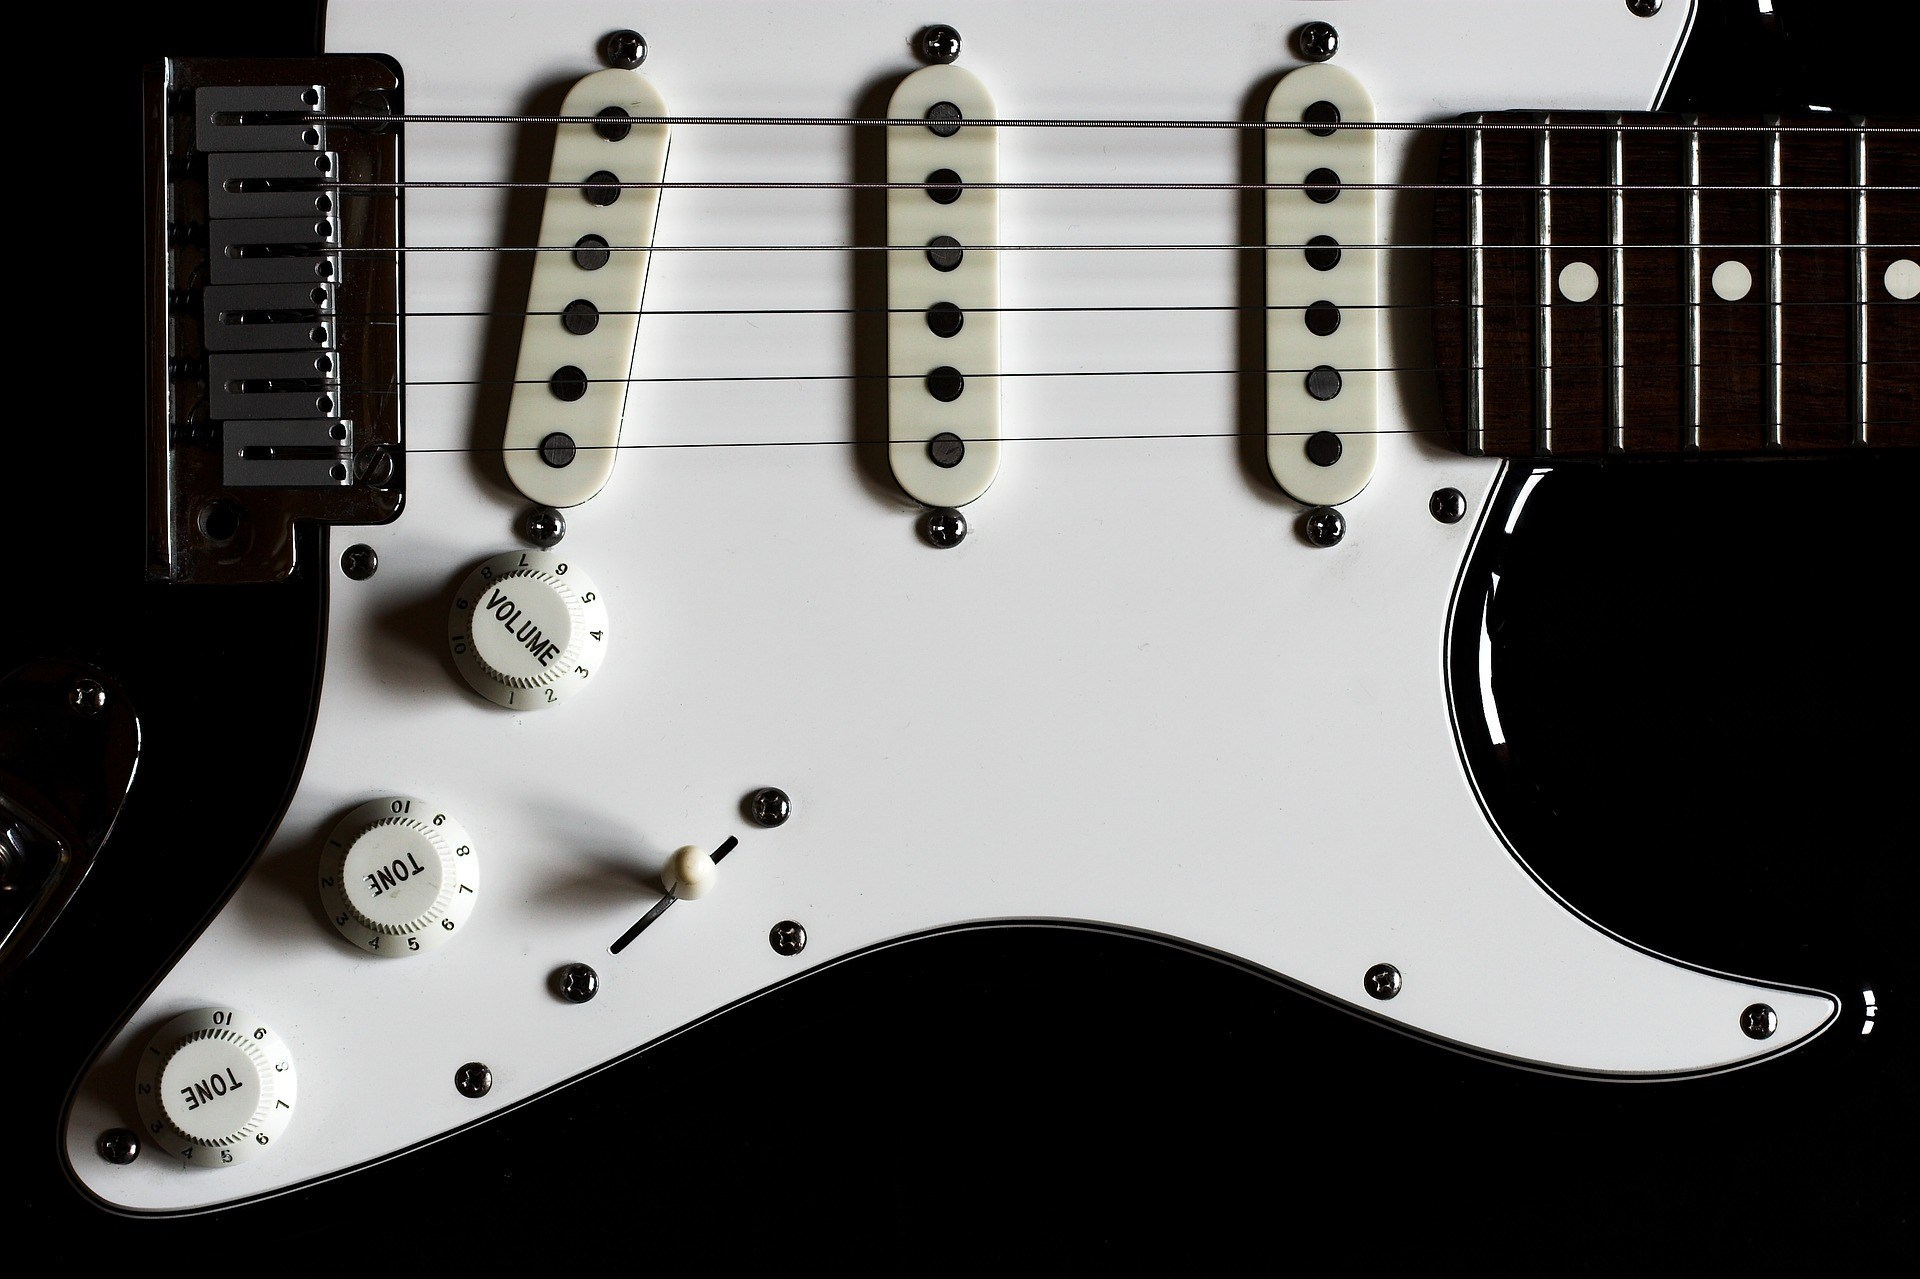
\includegraphics[width=\textwidth]{guitar2.png}

    \section{和弦选择?}
    当用户左手进行和弦选择时,红色框将在九宫格上滑动,来实时地反馈弹奏者手指地位置,当弹奏者\
    找到所需和弦时,降低左手位置超过一阈值就会触发和弦的设置。

    从交互角度来看,可以认为这是通过反馈来减少误选;
    从吉他弹奏角度来看,也可以理解成需要把弦按下力度达到一定程度才能达到效果,而不是轻碰就可以,\
    类似实际弹奏的逻辑。

    \section{弦的振动?}
    右手的操作我们也提供了反馈。可以看到界面上展示了吉他以及六根弦,当弹奏者右手触到相应位置时,\
    弦将给出合适的振动效果,使其看起来更加逼真。

    \section{后台运行?}
    后端的python脚本会持续运行处理并呈现数据,输出日志便于调试。下图是运行时的命令行窗口。
